\chapter{Graph-Färbung}

Im folgenden sei $ G = (V, E) $ ein fixierter Graph.

\begin{definition}[Coloring]
    Ein \textit{coloring} ist eine Funktion $ c : V \rightarrow \nats $ mit: wenn $ \{ u, v \} \in E $, dann $ c(u) \ne c(v) $.
\end{definition}

\begin{definition}[$ k $-Färbung]
    Ein Graph ist $ k $-färbbar, falls ein coloring $ c $ existiert mit $ |c(V)| \leq k $.
\end{definition}

\begin{definition}[Chromatische Zahl]
    Die chromatische Zahl $ \chi(G) $ eines Graphen ist definiert als das minimale $ k $, sodass $ G $ $ k $-färbbar ist.
\end{definition}

\begin{theorem}
    \label{thm:delta-coloring}
    Es gilt $ \chi(G) \leq \Delta(G) + 1 $.
\end{theorem}

\begin{proof}
    Färbe $ G $ greedy.
    Für $ v \in V $ mit $ v $ wurde noch nicht gefärbt, wähle die kleinste Farbe $ k \in \nats $, sodass kein Nachbar mit $ k $ gefärbt ist.
    Da jeder Knoten $ \Delta + 1 $ Nachbarn hat, ex. immer ein $ k \leq \Delta + 1 $, dass die Bedingung erfüllt.
\end{proof}

\begin{remark}
    Betrachte $ \{ v_1, \dots, v_{i - 1} \} \subseteq V $, die bereits greedy gefärbt wurden und Knoten $ v_i \in V $, der nun gefärbt werden soll.
    Für die Färbung von $ v_i $ werden maximal $ \deg_{G[\{ v_1, \dots, v_{i - 1} \}]}(v_i) + 1 $ Farben benötigt, nicht $ \deg(v_i) + 1 $.

    Der obige Algorithmus lässt sich also dahingehend verbessern, dass die Knoten nach Grad absteigend sortiert färbt.
\end{remark}

\begin{theorem}
    Für jeden Graph mit $ |E| = m $ gilt:
    \begin{equation*}
        \chi(G) \leq \frac{1}{2} + \sqrt{2m + \frac{1}{4}}
    \end{equation*}
\end{theorem}

\begin{proof}
    Sei $ c $ eine $ k $-Färbung mit $ k = \chi(G) $.
    Dann ex. mindestens eine Kante zwischen jeder Farbklasse.
    Andernfalls könnten zwei Klassen ohne Kante dieselbe Farbe nutzen.
    Also gilt:
    \begin{equation*}
        m \geq \frac{1}{2} \chi(G) (\chi(G) - 1)
    \end{equation*}
    Diese Gleichung kann entsprechend umgestellt werden.
\end{proof}

\begin{definition}[Clique]
    Eine Clique ist ein vollständiger verbundener (Teil-)Graph.
    $ K_\alpha $, $ \alpha \in \nats^+ $ bezeichnet den vollständigen Graphen mit $ \alpha $-vielen Knoten.
\end{definition}

\begin{proposition}
    Falls $ K_\alpha \subseteq G $, $ \alpha \in \nats^+ $, dann:
    \begin{equation*}
        \chi(G) \geq \alpha = \Delta(K_\alpha) + 1
    \end{equation*}
\end{proposition}

\begin{definition}[Odd-cycle]
    Sei $ C $ ein Kreis in $ G $.
    $ C $ ist ein \textit{odd-cycle}, falls $ |C| \mod 2 \ne 0 $.
\end{definition}

\begin{proposition}
    Gibt es einen odd-cycle in $ G $, gilt $ \chi(G) \geq 3 $.
\end{proposition}

\begin{lemma}
    \label{lem:min-deg-3-connected}
    Sei $ G $ 2-verbunden mit $ \delta(G) \geq 3 $.
    Falls $ G $ nicht vollständig ist, dann enthält $ G $ einen induzierten Pfad  $uvw $ auf 3 Knoten $ u, v, w \in V $, sodass $ G \setminus \{ u, w \} $ weiterhin verbunden ist.
\end{lemma}

\begin{proof}
    Da $ G $ verbunden aber nicht vollständig ist, ex. ein induzierter Pfad auf 3 Knoten.
    Falls $ G $ zusätzlich 3-verbunden ist, kann jeder solche Pfad für das Lemma gewählt werden.
    Es genügt daher, den Beweis nur für 2-verbundene Graphen zu führen.

    Sei $ \{ v, x\} \subseteq V $ ein cutset von $ G $.
    Dann ist $ G \setminus \{ v \} $ verbunden, aber nicht 2-verbunden und hat zwei Blöcken $ B_1, B_2 $.
    Somit ex. zwei non-cut-vertices $ u \in B_1 $ und $ w \in B_2 $ adjazent zu $ v $.
    $ uvw $ ist der gesuchte Pfad.
\end{proof}

\begin{theorem}[Brooks' Theorem ('41)]
    Jeder Graph hat ein $ \Delta(G) $-coloring, außer:
    \begin{enumerate}
        \item \label{itm:brooks-vollst}
        $ G $ enthält einen vollst. Teilgraphen $ K_{\Delta(G) + 1} $ oder
        \item \label{itm:brooks-odd}
        $ \Delta(G) = 2 $ und $ G $ enthält einen odd-cycle.
    \end{enumerate}
\end{theorem}

\begin{proof}
    Nach Lov\'{a}sz ('75).

    Sei $ G $ verbunden.
    Es gelte weder \ref{itm:brooks-vollst} noch \ref{itm:brooks-odd}.
    Beweis per Fallunterscheidung:
    \begin{enumerate}
        \item \label{itm:deg-le-delta}
        Angenommen, $ G $  enthält einen Knoten $ v \in V $ mit $ \deg(v) < \Delta(G) $.

        Färbe $ G $ greedy mit Reihenfolge der Knoten sortiert nach Distanz zu $ v $, d.h. $ v $ wird zuletzt und die am weitesten von $ v $ entfernten Knoten zuerst gefärbt.
        Es gilt dann für $ u \in V $ mit $ u \ne v $, dass ein Nachbar $ w $ zu $ u $ ex., der noch nicht gefärbt wurde.
        Es werden also max. $ \Delta $ Farben gebraucht (vgl. Theorem \ref{thm:delta-coloring}).

        Insbesondere gilt $ \deg(v) < \Delta $ und damit wird $ v $ korrekt gefärbt.

        \item Angenommen, es sei $ v \in V $ ein cut vertex in $ G $, d.h. $ G $ nicht 2-verbunden.

        Für jede zusammenhängende Menge an Knoten $ V' \subseteq V $ von $ G \setminus \{ v \} $ gilt: $ G[V' \cup \{ v \}] $ kann mit $ \Delta(G) $-vielen Farben gefärbt werden, dafür $ G[V' \cup \{ v \}] $ Fall \ref{itm:deg-le-delta} gilt.

        Eine Färbung für $ G $ kann erzeugt werden, indem die Farbklassen von den Komponenten $ V' $ je so permutiert werden, dass $ v $ immer gleich gefärbt wird.

        \item Sei $ G $ $ \Delta(G) $-regulär, d.h. $ \forall v \in V: \deg(v) = \Delta(G) $, 2-verbunden und nicht vollständig.

        Sei $ uvw $ ein Pfad nach Lemma \ref{lem:min-deg-3-connected}.
        Färbe $ u $ und $ w $ mit Farbe 1.
        Färbe $ G \setminus \{ u , w \} $ greedy absteigend nach Distanz zu $ v $; hier trifft wieder Fall \ref{itm:deg-le-delta} zu.

        Schlussendlich kann auch $ v $ gefärbt werden, da $ u $ und $ w $ die gleiche Farbe nutzen.
    \end{enumerate}
\end{proof}

\begin{lemma}
    \label{lem:planar-degree}
    Sei $ G $ ein planarer Graph, dann gilt für den durchschnittlichen Knotengrad $ d(G) $: $ d(G) < 6 $.
\end{lemma}

\begin{proof}
    Es gilt $ d(G) = 2 \frac{|E|}{|V|} $.
    Mit $ |V| \geq 3 $, $ |E| \leq 3 |V| - 6 $ (cgl. Korollar \ref{cor:max-edges}).
    Dann gilt:
    \begin{align*}
        d(G) & \leq \frac{2 \cdot (3|V| - 6)}{|V|} \\
        &= 6 - \frac{12}{|V|} < 6
    \end{align*}
\end{proof}

\begin{theorem}
    Jeder planare Graph hat $ \chi(G) \leq 6 $.
\end{theorem}

\begin{proof}
    Beweis per Induktion über $ |V| $.
    \begin{description}
        \item[IS] Für $ |V| \leq 6 $ trivial.
        \item[IV] Es gelte, ein Graph mit $ n $ Knoten ist 6-färbbar.
        \item[IS] Sei $ G $ ein planarer Graph mit $ |V| = n + 1 $.

        Nach Lemma \ref{lem:planar-degree} existiert ein Knoten $ w \in V $ mit $ \deg(w) \leq 5 $.
        Sei $ G' = G \setminus \{ w \} $.
        Nach IV ist $ G' $ 6-färbbar.
        Sei $ c $ eine solche 6-Färbung.

        Da $ w $ nur 5 Nachbarn in $ G' $ hat, ex. eine Farbe $ k $ mit der $ w $ gefärbt werden kann, also ist auch $ G $ 6-färbbar.
    \end{description}
\end{proof}

\begin{theorem}
    Für jeden planaren Graphen $ G $ gilt $ \chi(G) \leq 5 $.
\end{theorem}

\begin{proof}
    Färbe zunächst alle Knoten $ v \in V $ mit $ \deg(v) < 5 $ rekursiv und greedy.
    Sei $ c $ diese Färbung.
    Es kann angenommen werden, dass $ G $ einen Knoten $ v $ mit $ \deg(v) = 5 $ enthält; andernfalls ist der Beweis trivial.

    Für $ v_1, v_2 \in V $ sei $ V_{v_1, v_2} = \{ v \in V \mid c(v) \in \{ c(v_1), c(v_2) \} \} $ und $ V^*_{v_1, v_2} = \{ v \in V \mid $ es ex. Pfad von $ x $ nach $ v $ in $ V_{x, y} \} $.

    Betrachte $ x, y \in V $ mit $ c(x) \ne c(y) $.
    Fallunterscheidung:
    \begin{enumerate}
        \item \label{itm:case-color-xy}
        Angenommen, es ex. kein Pfad $ P $ in $ V_{x,y} $ von $ y $ nach $ x $.
        Dann gilt $ V^*_{x,y} \cap V^*_{y,x} = \emptyset $.

        Dann definiere neue Färbung $ c' $, die die Farben in $ V^*_{x, y} $ tauscht:
        \begin{equation*}
            c'(s) = \begin{cases}
                c(s), & s \notin V^*_{x, y}, \\
                c(x), & s \in V^*_{x,y}, c(s) \ne c(x) \\
                c(y), & s \in V^*{x,y}, c(s) = c(x)
            \end{cases}
        \end{equation*}

        Somit kann in $ v $ in $ c' $ auf $ c(x) $ gesetzt werden.

        \item Angenommen, es ex. ein Pfad $ P $ in $ V_{x,y} $ von $ x $ nach $ y $.

        Betrachte Nachbarn $ t, z \in V $ von $ v $; dargestellt in Abbildung \ref{fig:5-colorable}.
        Es gilt: $ V_{t,z} \cap V_{x,y} = \emptyset $.

        Dann muss gelten, dass $ V^*_{t,z} \cap V^*_{z,t} = \emptyset $ oder Widerspruch zu $ G $ ist planar.
        Somit lassen sich $ t $ und $ z $ nach Fall \ref{itm:case-color-xy} umfärben.
    \end{enumerate}

    \begin{figure}
        \centering
        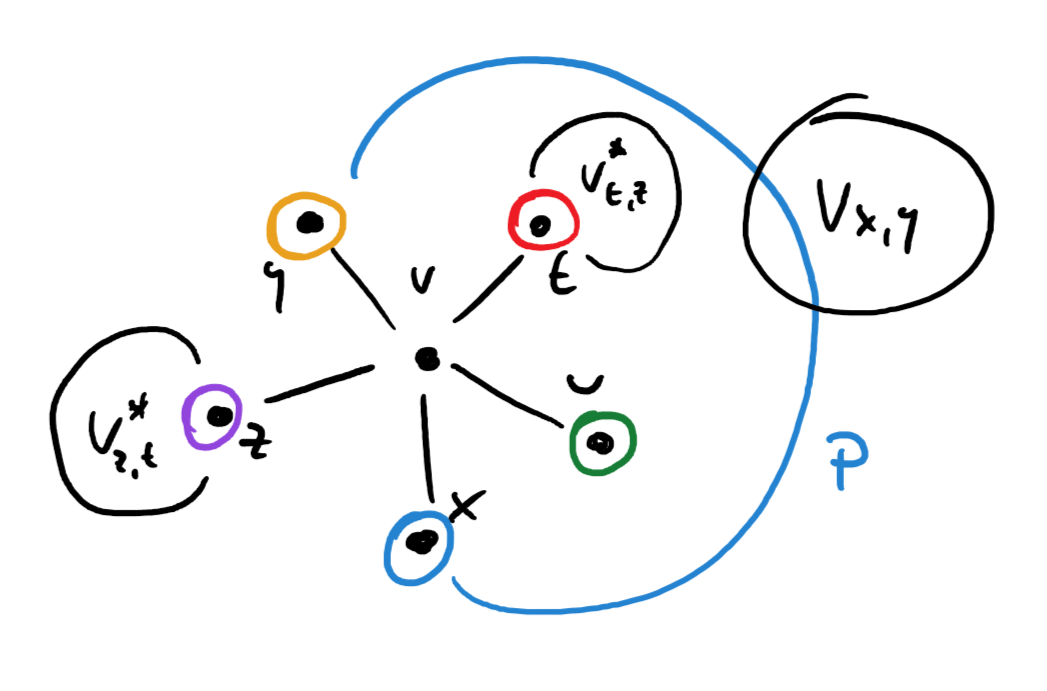
\includegraphics[width=0.45\textwidth]{figures/5-colorable.png}
        \caption{Beweis 5-Farbensatz Veranschaulichung}
        \label{fig:5-colorable}
    \end{figure}
\end{proof}
